\documentclass{report}
\usepackage[english]{babel}
\usepackage{placeins}
\usepackage[utf8]{inputenc}
\usepackage{multicol}
\usepackage{multirow}
\usepackage{url}
\usepackage{graphicx}
\usepackage{amsfonts}
\usepackage[tbtags]{amsmath}
\usepackage{amsmath}
\usepackage{caption}
\usepackage{subcaption}
\usepackage{float}
\usepackage[letterpaper,top=2cm,bottom=2cm,left=3cm,right=3cm,marginparwidth=1.75cm]{geometry}
\usepackage{amsmath}
\usepackage{graphicx}
\usepackage[colorlinks=true, allcolors=blue]{hyperref}

\title{
	\endgraf\bigskip
	
	\begin{center}
		\Huge {{Report on Security Tool: ELK Stack} }\\\\
		\vspace{0.5cm}
		\large {CSE406: Computer Security Sessional}
	\end{center}
	\bigskip
	\bigskip
}

\author{
    \large{Kazi Ababil Azam (1805077)}\\
	\large{Fardin Anam Aungon (1805087)}\\
	\large{Department of Computer Science and Engineering}\\
    \large{Bangladesh University of Engineering and Technology (BUET)}
}

\date{
	\endgraf\bigskip
	\Large{\today}
}

\begin{document}
\maketitle
\tableofcontents

% Report starts

\chapter{Introduction}

\section{What is ELK Stack?}
ELK Stack is a combination of three open source projects: Elasticsearch, Logstash, and Kibana. 
ELK Stack is most commonly used for log aggregation and log analysis. The ELK Stack is a great collection
of tools to collect, analyze and visualize data. It is a very powerful stack that provides developers and
system operators with great insights into their operational data.


%insert layer image of ELK Stack here
\begin{figure}[h]
	\centering
	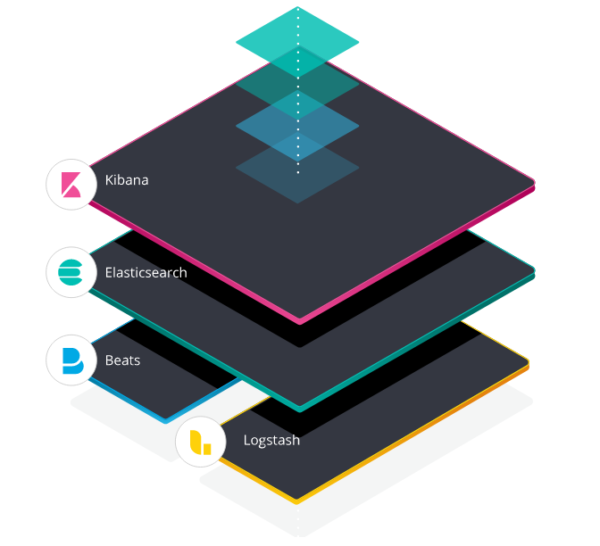
\includegraphics[width=0.7\textwidth]{Images/ELK_Layers.png}
	\caption{ELK Stack}
	\label{fig:Components of ELK Stack}
\end{figure} 

\chapter{General Overview of ELK Stack}
\section{Components of ELK Stack}
ELK Stack is mainly composed of three components:
\begin{itemize}
	\item Elasticsearch, the search and analytics engine
	\item Logstash, the data processing pipeline
	\item Kibana, the data visualization tool
\end{itemize}

% enter image of ELK Stack here
\begin{figure}[h]
	\centering
	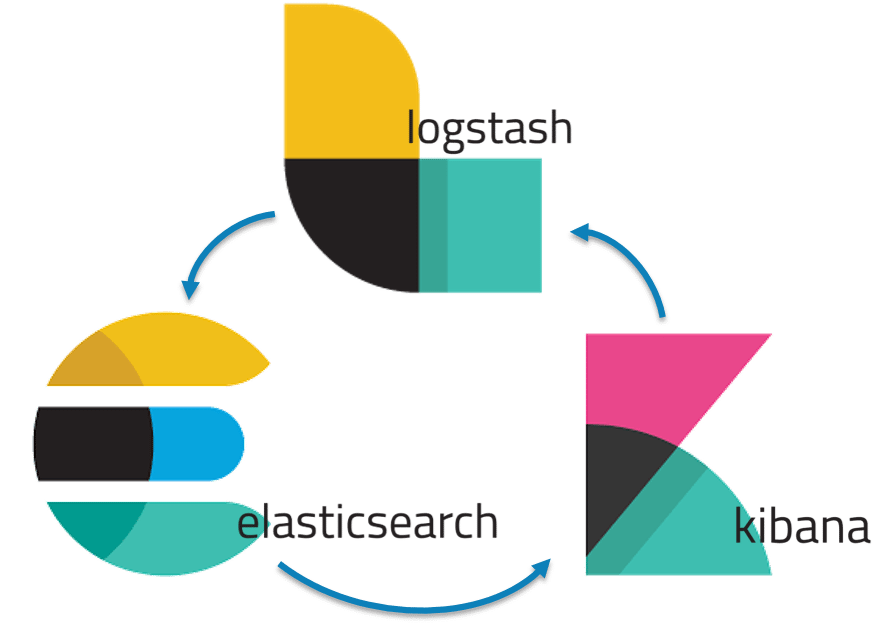
\includegraphics[width=0.7\textwidth]{Images/ELK.png}
	\caption{Components of ELK Stack}
	\label{fig:ELK Stack}
\end{figure}

\subsection*{Elasticsearch}
Elasticsearch is the centralized component of the Elastic Stack.
It is a distributed, RESTful search and analytics engine capable of solving a growing number of use cases.
It is based on a server that can process JSON requests, index documents containing JSON objects, and give back JSON responses.
Using a structure based on documents instead of tables, it is able to provide a scalable search solution with a low latency, and 
comes with extensive REST APIs for storing and searching the data.

\subsection*{Logstash}
Logstash is a open-source, server-side data processing pipeline which ingests data from multiple sources simultaneously. 
It has roughly 3 stages in its working principle.
\begin{itemize}
	\item Input: listen for and accept log data
	\item Filter: filter, parse and enrich the log data
	\item Output: sends the log to another system
\end{itemize}

\subsection*{Kibana}
Kibana is basically a data visualization and management tool. It lets users visualize the data handled by Elastisearch and 
navigate the stack. All it needs is an index to search through the data. 
It is a web application that runs on top of Elasticsearch.

\section{Working Principle of ELK Stack}

The working principle of ELK Stack is shown below:

% insert image of working principle of ELK Stack here
\begin{figure}[h]
	\centering
	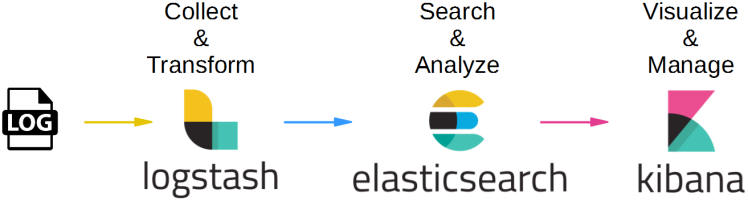
\includegraphics[width=\textwidth]{Images/ELK_Working_Principle.png}
	\caption{Working Principle of ELK Stack}
	\label{fig:Working Principle of ELK Stack}
\end{figure}

\section{Features of ELK Stack}
\begin{itemize}
	\item Open-source and Scalable
	\item Full-stack monitoring support
	\item Index based search
	\item Real-time data analysis
	\item Provides security solution through different integrations
\end{itemize}

\section{SIEM components}
SIEM means Security Information and Event Management. It delves into log records and real-time data to 
provide security intelligence for monitoring, event correlation, and incident response. SIEM is a combination of two technologies:
\begin{itemize}
	\item Security Information Management (SIM): log records and event data
	\item Security Event Management (SEM): real-time monitoring and correlation of events
\end{itemize}

\section{SIEM with ELK Stack}
The way how SIEM works with ELK Stack is described as follows:
\begin{figure}[ht]
	\centering
	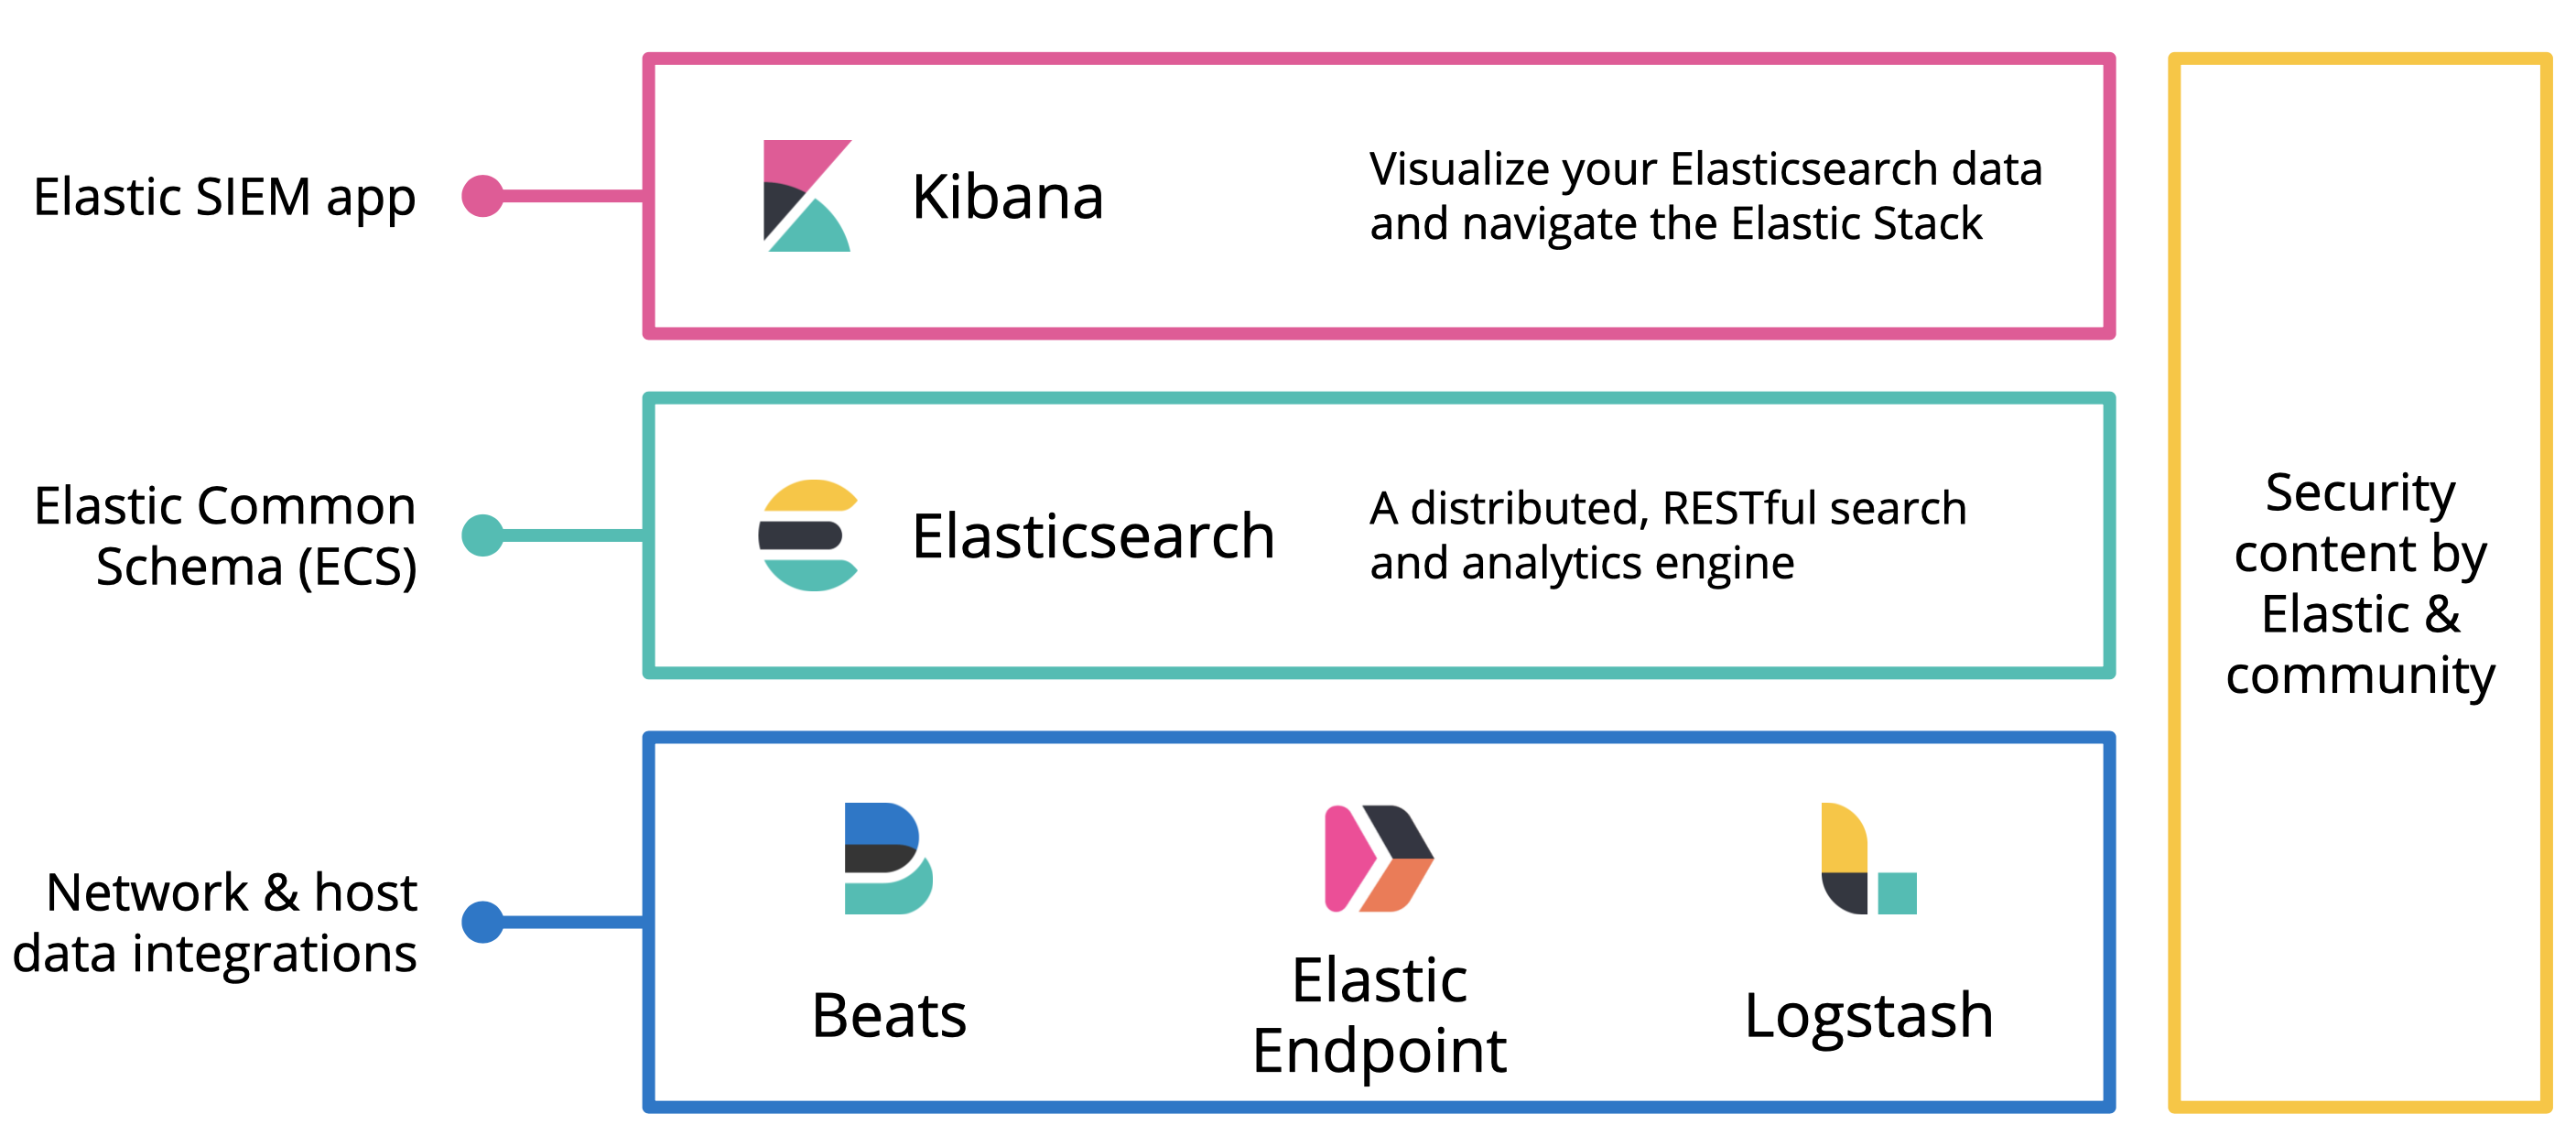
\includegraphics[width=\textwidth]{Images/SIEM.png}
	\caption{SIEM with ELK Stack}
	\label{fig:SIEM with ELK Stack}
\end{figure}

\begin{itemize}
	\item \textbf{Elastic Endpoint Security} is an endpoint security platform and agent that provides prevention, detection, 
	and response capabilities. It ships events and security alerts directly to Elasticsearch.
	\item \textbf{Beats} are open source data shippers that you install as agents on your systems. 
	Beats send security events and other data to Elasticsearch.
	\item \textbf{Elasticsearch} excels at indexing streams of semi-structured data, 
	such as logs or metrics, while \textbf{Kibana} is used to search, view, and interact with data stored in Elasticsearch indices. 
	You can easily perform advanced data analysis and visualize your data in a variety of charts, tables, and maps.
\end{itemize}

SIEM enables analysis of host-related and network-related security events as part of 
alert investigations or interactive threat hunting.

The SIEM app provides an interactive workspace for security teams to \textbf{triage events} 
and \textbf{perform initial investigations}. 
Additionally, machine learning anomaly detection jobs and detection engine rules provide ways to 
\textbf{automatically detect suspicious activity} across a entire fleet of servers and workstations. 
It is now a part of the generalized Elastic Security solution. 
Elastic Security is highly customizable and can be adapted to various security use cases, 
making it a popular choice for organizations looking to enhance their security posture. 
It's used by security teams to monitor and respond to security incidents, 
investigate threats, and gain insights into their infrastructure's security.

\chapter{Elastic Security Workflow}

\section{Elastic Security}
Elastic Security combines SIEM threat detection features with endpoint prevention and response capabilities in one solution. 
These analytical and protection capabilities, leveraged by the speed and extensibility of Elasticsearch, 
enable analysts to defend their organization from threats.

Elastic Security provides the following security benefits and capabilities:
\begin{itemize}
	\item A detection engine to identify attacks and system misconfigurations
	\item A workspace for event triage and investigations
	\item Interactive visualizations to investigate process relationships
	\item Inbuilt case management with automated actions
	\item Detection of signatureless attacks with prebuilt machine learning anomaly jobs and detection rules
\end{itemize}

\section{Elastic Security Components and Workflow}
A comprehensive diagram of the Elastic Security components and workflow is shown below:
\begin{figure}[ht]
	\centering
	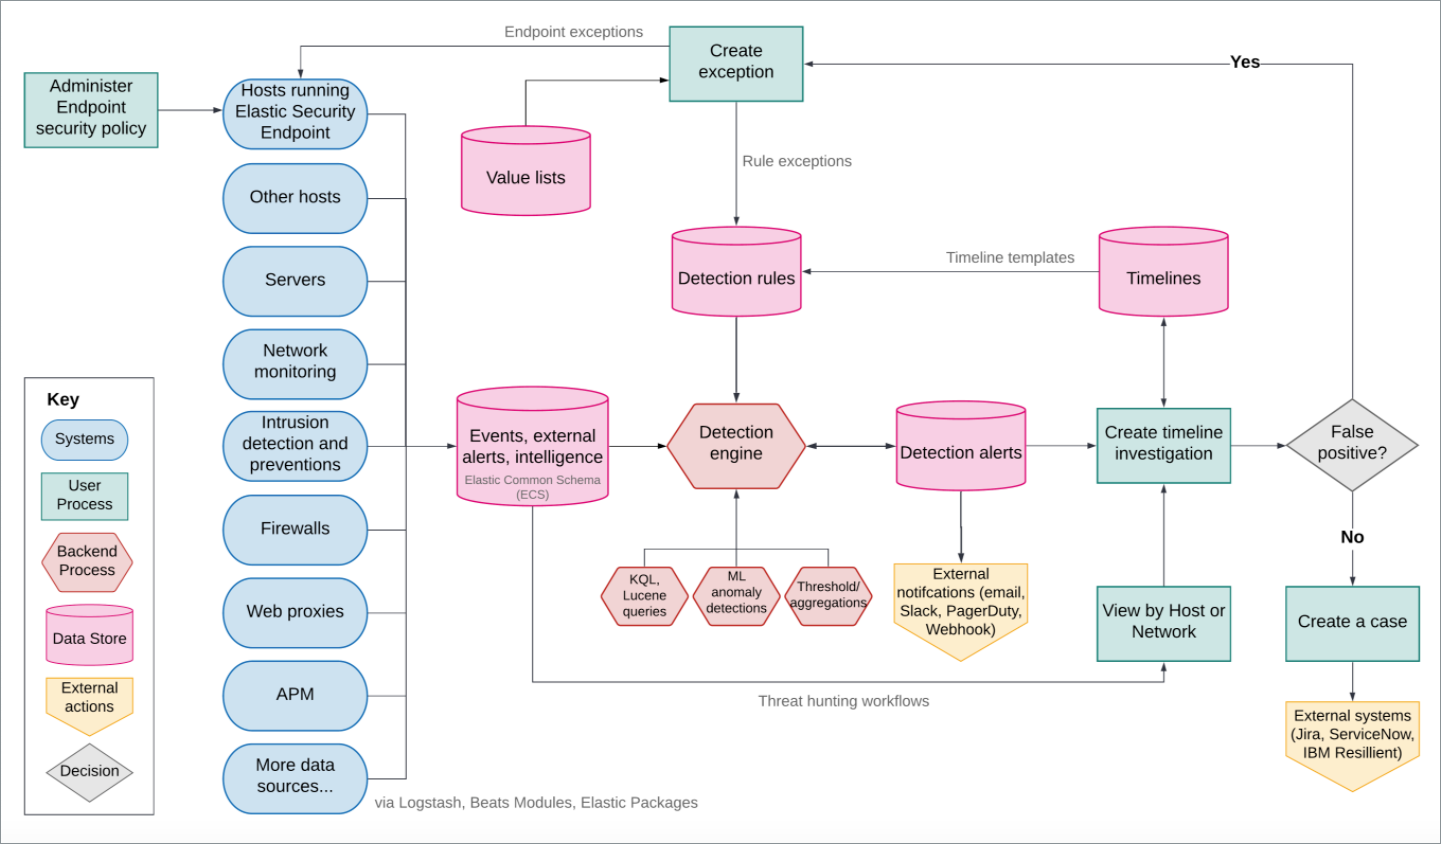
\includegraphics[width=0.87\textwidth]{Images/Security_Workflow.png}
	\caption{Elastic Security Components and Workflow}
	\label{fig:Elastic Security Components and Workflow}
\end{figure}

Here's an overview of the flow and its components:

\begin{itemize}
	\item Data is shipped from your hosts to Elasticsearch in the following ways:
	\begin{itemize}
		\item \textbf{Elastic Defend:} Elastic Agent integration that protects your hosts against malware and ships these data sets:
		\begin{itemize}
			\item Windows: Process, network, file, DNS, registry, DLL and driver loads, malware security detections
			\item Linux/macOS: Process, network, file
		\end{itemize}
		\item \textbf{Integrations:} Integrations are a streamlined way to send your data to the Elastic Stack. 
		Integrations are available for popular services and platforms, like Nginx, AWS, and MongoDB, 
		as well as many generic input types like log files.
		\item \textbf{Beat modules:} Beats are lightweight data shippers. 
		Beat modules provide a way of collecting and parsing specific data sets from common sources, such as cloud and OS events, logs, and metrics.
	\end{itemize}
	\item The Elastic Security app in Kibana is used to manage the \textbf{Detection engine}, \textbf{Cases}, and \textbf{Timeline}, 
	as well as administer hosts running Elastic Defend:
	\begin{itemize}
		\item \textbf{Detection engine:} Automatically searches for suspicious host and network activity via the following:
		\begin{itemize}
			\item \textbf{Detection rules:} Periodically search the data (Elasticsearch indices) sent from your hosts for 
			suspicious events. 
			When a suspicious event is discovered, an alert is generated.
			\item \textbf{Exceptions:} Reduce noise and the number of false positives. 
			Exceptions are associated with rules and prevent alerts when an exception's conditions are met. 
			Value lists contain source event values that can be used as part of an exception's conditions. 
			\item \textbf{Machine learning jobs:} Automatic anomaly detection of host and network events.
			Anomaly scores are provided per host and can be used with detection rules.
		\end{itemize}
		\item \textbf{Cases:} An internal system for opening, tracking, and sharing security issues directly in the Security app. 
		Cases can be integrated with external ticketing systems.
		\item \textbf{Timeline:} Workspace for investigating alerts and events. 
		Timelines use queries and filters to drill down into events related to a specific incident.
		Timeline templates are attached to rules and use predefined queries when alerts are investigated.
		Timelines can be saved and shared with others, as well as attached to Cases.
		\item \textbf{Administration:} View and manage hosts running Elastic Defend.
	\end{itemize}
\end{itemize}

\chapter{Features to be Demonstrated}
The SIEM features for different contexts are implemented through integrations installed in the cloud deployment 
(which we are accessing through the free trial) od Elastic Security.
The features that we are going to demonstrate are as follows:
\begin{itemize}
	\item \textbf{Network Packet Capture:} displays flow information about network connections on a host.
	\item need to add
\end{itemize}

\chapter{Demonstration}
\section{Elastic Cloud: Sign up}
The first step is to create an Elastic Cloud deployment. 
We can create a free trial deployment by signing up for a free trial account.
\begin{itemize}
	\item Go to \url{https://cloud.elastic.co/registration?elektra=guide-welcome-cta}.
	\item Sign up or log in.
	\begin{figure}[!h]
		\centering
		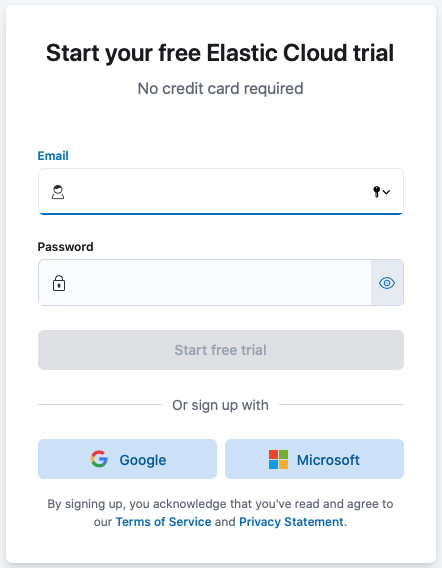
\includegraphics[width=0.5\textwidth]{Images/sign-up-trial.png}
		\caption{Sign Up}
		\label{fig:Sign Up}
	\end{figure}
	\item Create a deployment.
	\begin{figure}[!h]
		\centering
		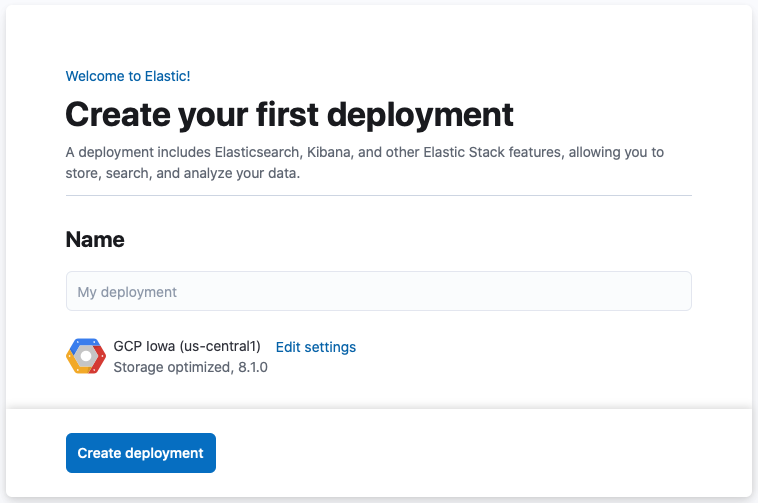
\includegraphics[width=0.5\textwidth]{Images/create-first-deployment.png}
		\caption{Create Deployment}
		\label{fig:Create Deployment}
	\end{figure}
	\item Save your elastic superuser credentials.
	\begin{figure}[!h]
		\centering
		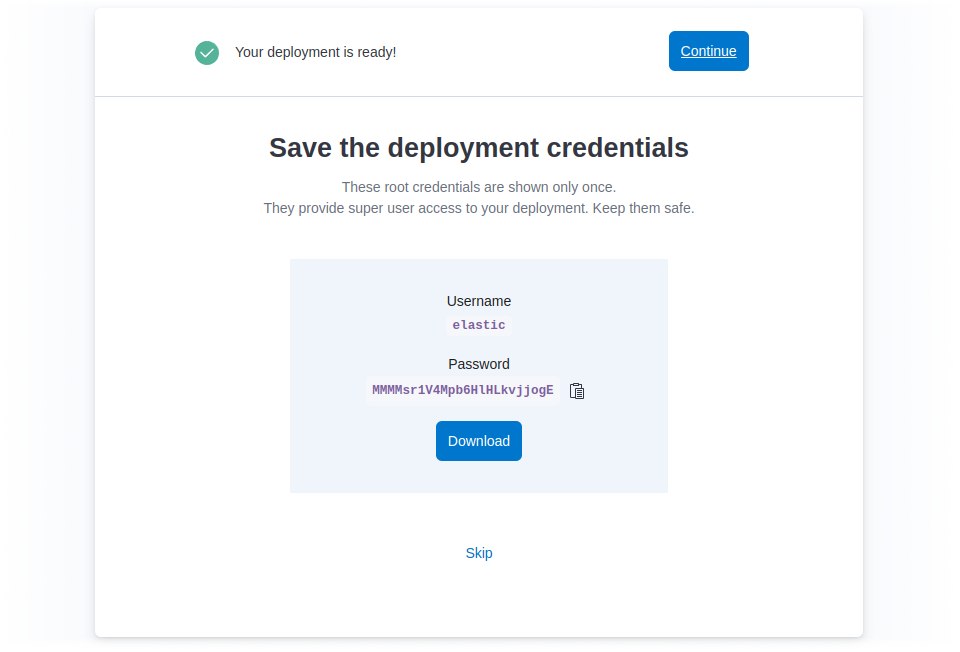
\includegraphics[width=0.7\textwidth]{Images/elastic-password.png}
            \caption{Save Superuser Credentials}
		\label{fig:Save Superuser Credentials}
	\end{figure}
	\item Once the deployment is ready, select continue.
\end{itemize}

The deployment includes a pre-configured instance of Fleet Server, 
which manages the Elastic Agents that can be used to monitor a host system.

\section{Adding the integration}
\begin{itemize}
	\item Log in to your cloud deployment, which will take you to Kibana Home.
	\item Click Add Integrations.
	\item Search and select the 'Network Packet Capture' integration.
	\item Click add and configure the integration with the following details:
	\begin{itemize}
		\item Integration name: Give the integration a name.
		\item Description: Enter a brief description of the integration.
		\item New agent policy name: Since you'll be creating a new agent policy, enter a name to identify it. 
		Ensure that you leave the Collect system logs and metrics option selected.
	\end{itemize}
	Click Save and continue to proceed.
	\item Click Add Elastic Agent to your hosts.
\end{itemize}

\section{Adding an agent}
\begin{itemize}
	\item Follow the Install Elastic Agent on you host step. 
	Pick the appropriate operating system and download and install your agent.
	\item Once the agent is installed, the agent will automatically enroll with the Fleet Server.
	It is shown in the Agent enrollment confirmed step.
	\item Click on Add the integration at the bottom of the screen to proceed.
	\item The only step remaining is to confirm the incoming data. Click on confirm and it will show a preview of the 
	data Kibana is receiving.
	\item Click on View Assets to show the Dashboards under Network Packet Capture integration.
\end{itemize}

\section{Dashboards}
The dashboards are prepared using the data received from the agents installed in the host. 
They are prepared using Kibana.
The different dashboards we can visualize the packet data with are:
\begin{itemize}
	\item Overview
	\item DNS Overview
	\item DHCPv4
	\item Cassandra
	\item Network Flows
	\item HTTP
	\item MongoDB
	\item MySQL
	\item NFS
	\item PostgreSQL
	\item Thrift
	\item TLS Sessions
\end{itemize}
Here are some of the screenshots taken of the dashboards.


\end{document}

